\documentclass[
	letterpaper, % Paper size, specify a4paper (A4) or letterpaper (US letter)
	10pt, % Default font size, specify 10pt, 11pt or 12pt
]{CSUniSchoolLabReport}

%----------------------------------------------------------------------------------------
%	REPORT INFORMATION
%----------------------------------------------------------------------------------------

\title{Lab Five\\ Power Systems Analysis \\ EECE5682} % Report title

\author{Michael \textsc{Brodskiy}\\ \small \href{mailto:Brodskiy.M@Northeastern.edu}{Brodskiy.M@Northeastern.edu}}

\date{November 12, 2024} % Date of the report

%----------------------------------------------------------------------------------------


\begin{document}

\maketitle % Insert the title, author and date using the information specified above

\begin{center}
	\begin{tabular}{l r}
		Date Performed: & \today \\ % Date the experiment was performed
		Instructor: & Professor \textsc{Abur} \\ % Instructor/supervisor
	\end{tabular}
\end{center}

\newpage

\begin{abstract}

  This laboratory experiment orients the performer with the Power Education Toolbox (PET) program. Furthermore, the experiment solidifies concepts related to bus-based systems, including power flow solutions, generation of an admittance matrix, and the affects of connecting/disconnecting components.

\end{abstract}

\begin{flushleft}

  \textsc{Keywords:} \underline{PET}, \underline{bus}, \underline{power flow}, \underline{admittance matrix}

\end{flushleft}

\newpage

\section{Introduction \& Objectives}

We begin by constructing the provided 5-bus system in the Power Education Toolbox (PET) program. The system looks as follows:

\begin{figure}[H]
  \centering
  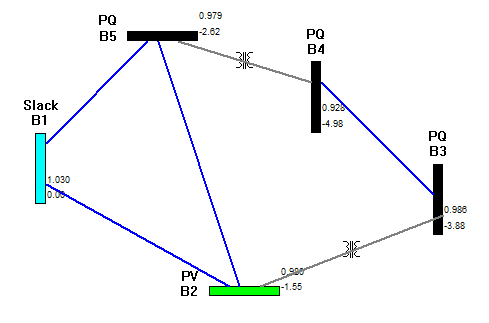
\includegraphics[width=.9\textwidth]{Figures/Lab\ Five/System.png}
  \caption{The Five-Bus System}
  \label{fig:1}
\end{figure}

\section{Results}

The Results sown in Parts (1-4) are obtained from the data files generated by PET.

\subsection{Part 1}

\begin{figure}[H]
  \centering
  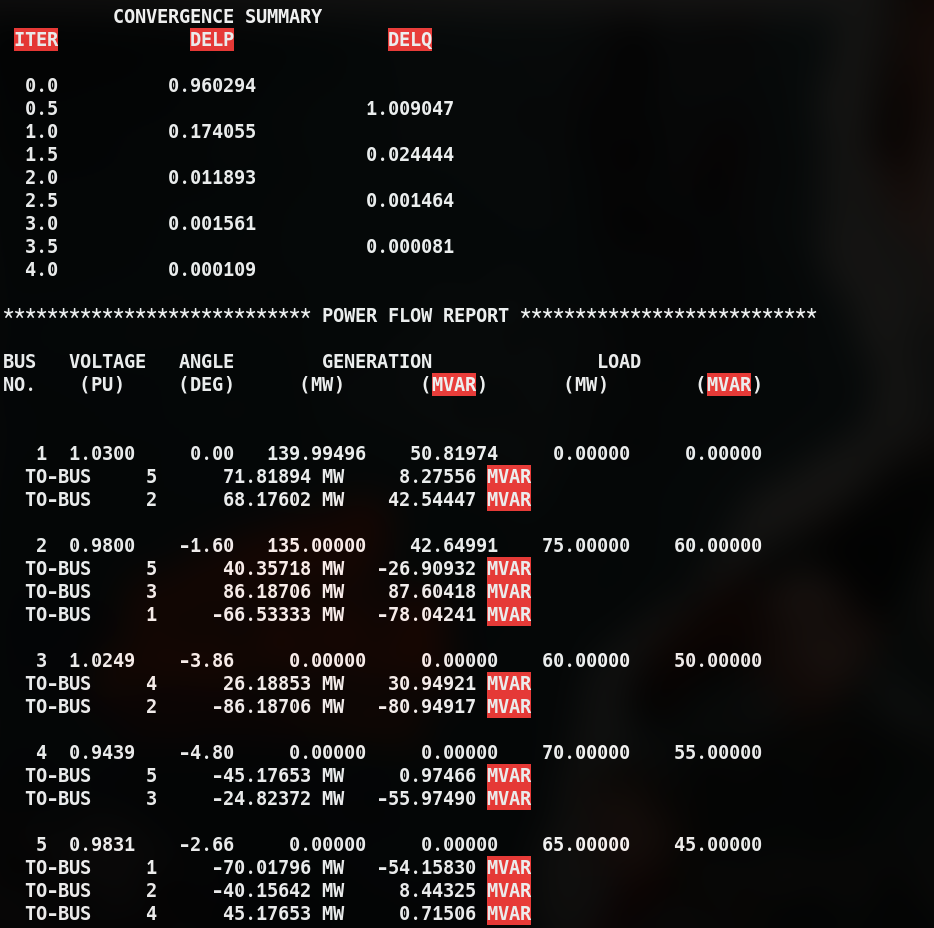
\includegraphics[width=.7\textwidth]{Figures/Lab\ Five/PF1}
  \caption{Power Flow — Part 1}
  \label{fig:2}
\end{figure}

\begin{figure}[H]
  \centering
  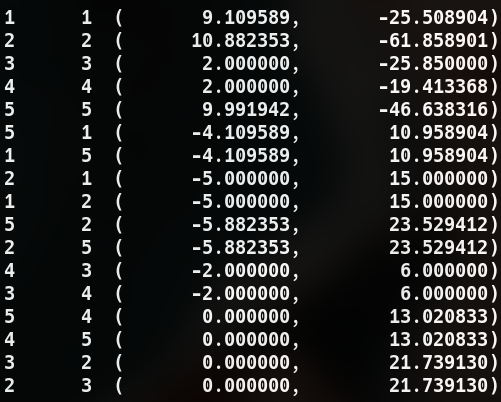
\includegraphics[width=.7\textwidth]{Figures/Lab\ Five/YMat1}
  \caption{$Y_{Bus}$ — Part 1}
  \label{fig:3}
\end{figure}

\subsection{Part 2}

\begin{figure}[H]
  \centering
  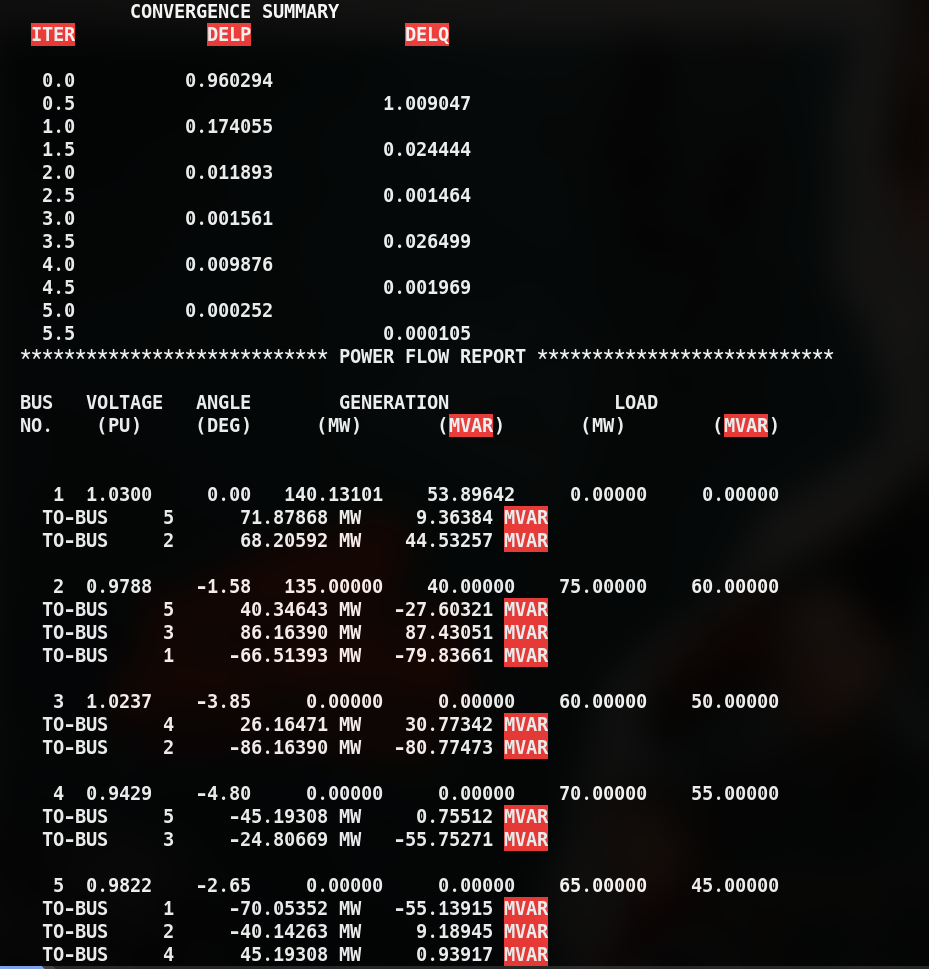
\includegraphics[width=.7\textwidth]{Figures/Lab\ Five/PF2}
  \caption{Power Flow — Part 2}
  \label{fig:4}
\end{figure}

\begin{figure}[H]
  \centering
  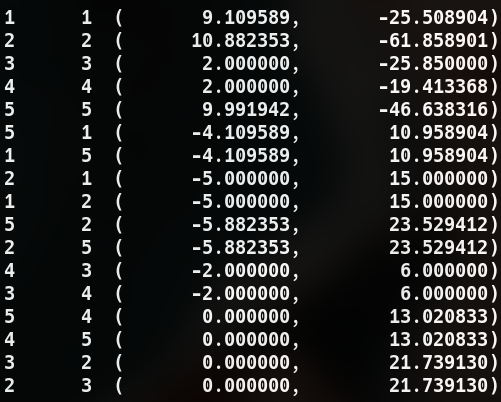
\includegraphics[width=.7\textwidth]{Figures/Lab\ Five/YMat2}
  \caption{$Y_{Bus}$ — Part 2}
  \label{fig:5}
\end{figure}

\subsection{Part 3}

\begin{figure}[H]
  \centering
  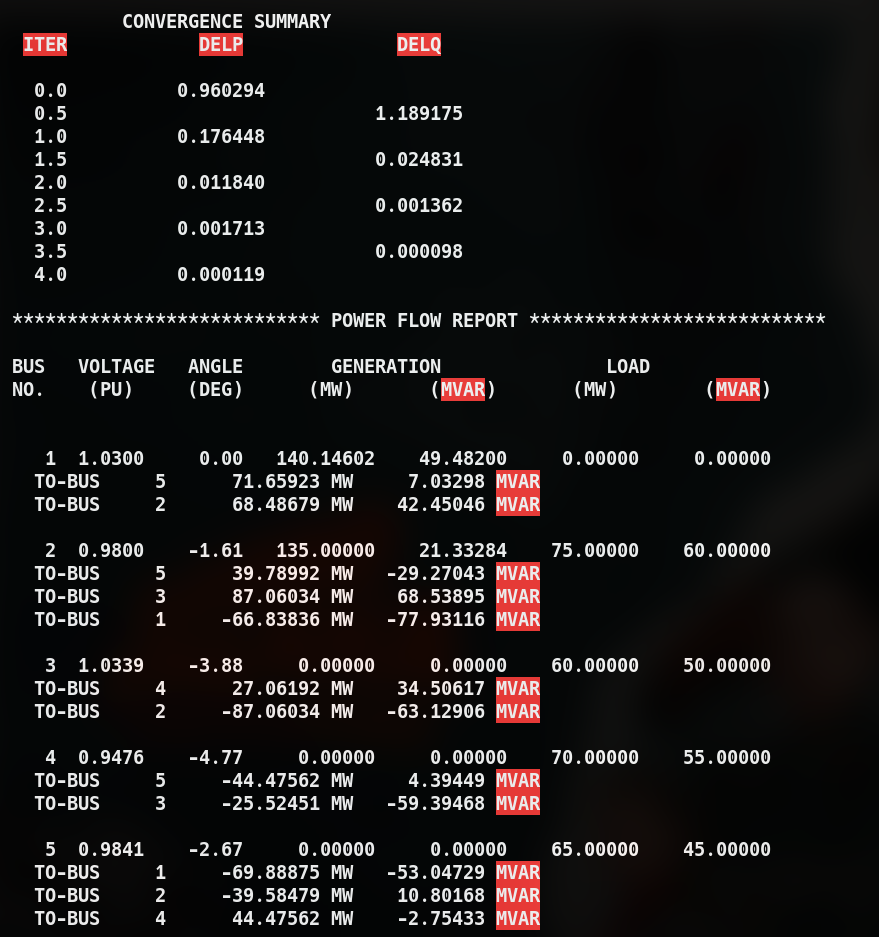
\includegraphics[width=.7\textwidth]{Figures/Lab\ Five/PF3}
  \caption{Power Flow — Part 3}
  \label{fig:6}
\end{figure}

\begin{figure}[H]
  \centering
  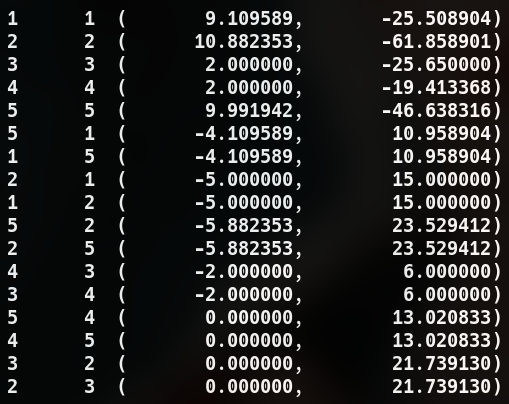
\includegraphics[width=.7\textwidth]{Figures/Lab\ Five/YMat3}
  \caption{$Y_{Bus}$ — Part 3}
  \label{fig:7}
\end{figure}

\subsection{Part 4}

\begin{figure}[H]
  \centering
  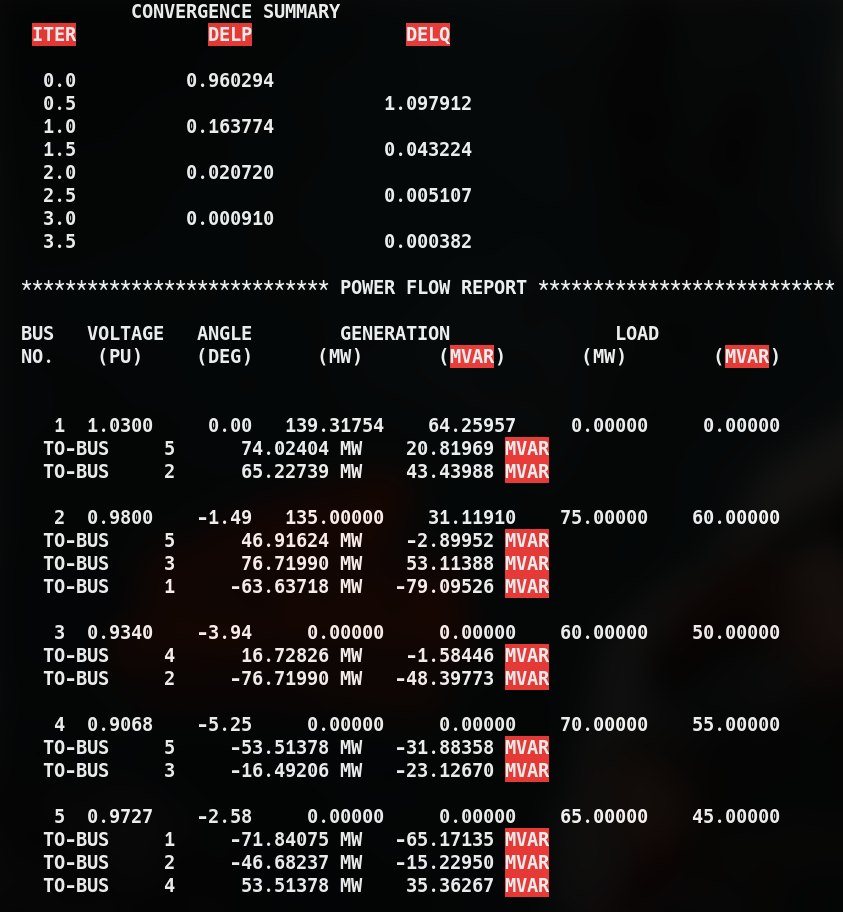
\includegraphics[width=.7\textwidth]{Figures/Lab\ Five/PF4}
  \caption{Power Flow — Part 4}
  \label{fig:8}
\end{figure}

\begin{figure}[H]
  \centering
  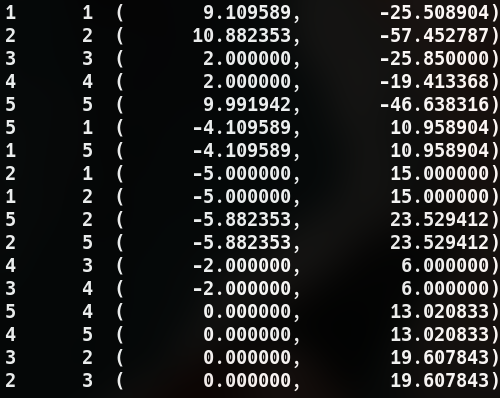
\includegraphics[width=.7\textwidth]{Figures/Lab\ Five/YMat4}
  \caption{$Y_{Bus}$ — Part 4}
  \label{fig:9}
\end{figure}

\subsection{Part 5}

Experimentally, we tweak the values of the real power load to find the point at which the power flow diverges. When changing by $50[\si{\mega\watt}]$, we see that this occurs at $420[\si{\mega\watt}]$. Changing values slightly, we observe that the power flow diverges for $P_L\geq 409[\si{\mega\watt}]$

\subsection{Part 6}

Now modifying to the power constraints for bus 2, as specified in Part (2), we find that the power flow diverges for $P_L\geq 388[\si{\mega\watt}]$.

\subsection{Part 7}

For the power flow to not diverge, we need at least $.34[p.u.]$ shunt capacitance. We slowly increase this value to find that, to maintain a bus voltage greater than $.9[p.u.]$ at a $400[\si{\mega\watt}]$ real load, with power constraints from Part (2), the shunt capacitance must be at least $1.51[p.u.]$.

\section{Analysis}

\subsection{Constructing $Y_{bus}$}

We may begin by constructing an admittance matrix based on the provided parameters. First and foremost, we may determine the zero parameters based on disconnected buses:

$$Y_{bus}=\left[ \begin{matrix} - & - & 0 & 0 & -\\ - & - & - & 0 & -\\ 0 & - & - & - & 0\\ 0 & 0 & - & - & -\\ - & - & 0 & - & - \end{matrix} \right]$$

From here, we find the off-diagonal elements by taking the inverse of the impedance. This gives us:

$$y_{12}=y_{21}=-\frac{1}{.02+.06j}=-5+15j$$
$$y_{15}=y_{51}=-\frac{1}{.03+.08j}=-4.1096+10.9589j$$
$$y_{23}=y_{32}=-\frac{1}{(.92)(.05j)}=21.739j$$
$$y_{25}=y_{52}=-\frac{1}{.01+.04j}=-5.8824+23.5294j$$
$$y_{34}=y_{43}=-\frac{1}{.05+.15j}=-2+6j$$
$$y_{45}=y_{54}=-\frac{1}{(.96)(.08j)}=13.021j$$

Putting this into our matrix, we get:

$$Y_{bus}=\left[ \begin{matrix} - & -5+15j & 0 & 0 & -4.1096+10.9589j\\ -5+15j & - & 21.739j & 0 & -5.8824+23.5294j\\ 0 & 21.739j & - & -2+6j & 0\\ 0 & 0 & -2+6j & - & 13.021j\\ -4.1096+10.9589j & -5.8824+23.5294j & 0 & 13.021j & - \end{matrix} \right]$$

Finally, we determine the diagonal terms:

$$y_{11}=-y_{12}-y_{15}+\frac{(B_{12}+B_{15})j}{2}=9.0196-25.5089j$$

Using a similar method, we get:

$$y_{22}=10.882-61.859j$$
$$y_{33}=2-25.85j$$
$$y_{44}=2-19.413j$$
$$y_{55}=9.992-46.638j$$

This gives us the final bus matrix (for parts 1 and 2) as:

$$\boxed{\left[ \begin{matrix} 9.0196-25.5089j & -5+15j & 0 & 0 & -4.1096+10.9589j\\ -5+15j & 10.882-61.859j & 21.739j & 0 & -5.8824+23.5294j\\ 0 & 21.739j & 2-25.85j & -2+6j & 0\\ 0 & 0 & -2+6j & 2-19.413j & 13.021j\\ -4.1096+10.9589j & -5.8824+23.5294j & 0 & 13.021j & 9.992-46.638j \end{matrix} \right]}$$

We may observe that this is in line with the generated buses from the results section. With the connection of the shunt capacitor in part (3), we modify the bus to get:

$$\boxed{\left[ \begin{matrix} 9.0196-25.5089j & -5+15j & 0 & 0 & -4.1096+10.9589j\\ -5+15j & 10.882-61.859j & 21.739j & 0 & -5.8824+23.5294j\\ 0 & 21.739j & 2-25.65j & -2+6j & 0\\ 0 & 0 & -2+6j & 2-19.413j & 13.021j\\ -4.1096+10.9589j & -5.8824+23.5294j & 0 & 13.021j & 9.992-46.638j \end{matrix} \right]}$$

Finally, changing the tap in part (4) would result in:

$$\boxed{\left[ \begin{matrix} 9.0196-25.5089j & -5+15j & 0 & 0 & -4.1096+10.9589j\\ -5+15j & 10.882-57.453j & 19.608j & 0 & -5.8824+23.5294j\\ 0 & 19.608j & 2-25.65j & -2+6j & 0\\ 0 & 0 & -2+6j & 2-19.413j & 13.021j\\ -4.1096+10.9589j & -5.8824+23.5294j & 0 & 13.021j & 9.992-46.638j \end{matrix} \right]}$$

We may see that the constructed buses match those generated in PET, with small variations due to rounding.

\subsection{Conclusions}

First and foremost, we may see that the admittance matrix simulated is precisely as expected. From parts one to two, there is no difference since no new components are connected. For part three, the addition of a shunt capacitor causes a shift in bus 3's diagonal term. For part 4, the change in the tap value of the transform causes a change in bus 2 and bus 3's values.

For the power flow, we may observe that, transitioning from part one to two, as expected, the generator from bus 1 must pick up the slack caused by stricter limitations on bus 2's reactive power flow. Furthermore, as expected, we may see that the addition of a shunt capacitor in part 3 changes very little for the real power flow; however, the reactive power flow to bus 3 decreases, while it increases for the other buses. Conversely, the increase of the tap in part 4 results in decreased real power flow to bus 3, while the real power flow to other buses increases (with little change in reactive power flow). As such, we see that the PET program does a great job of simulating bus responses to changes in power flow set up.

\subsection{Voltage Magnitude versus Real Power Load}

\begin{figure}[H]
  \centering
  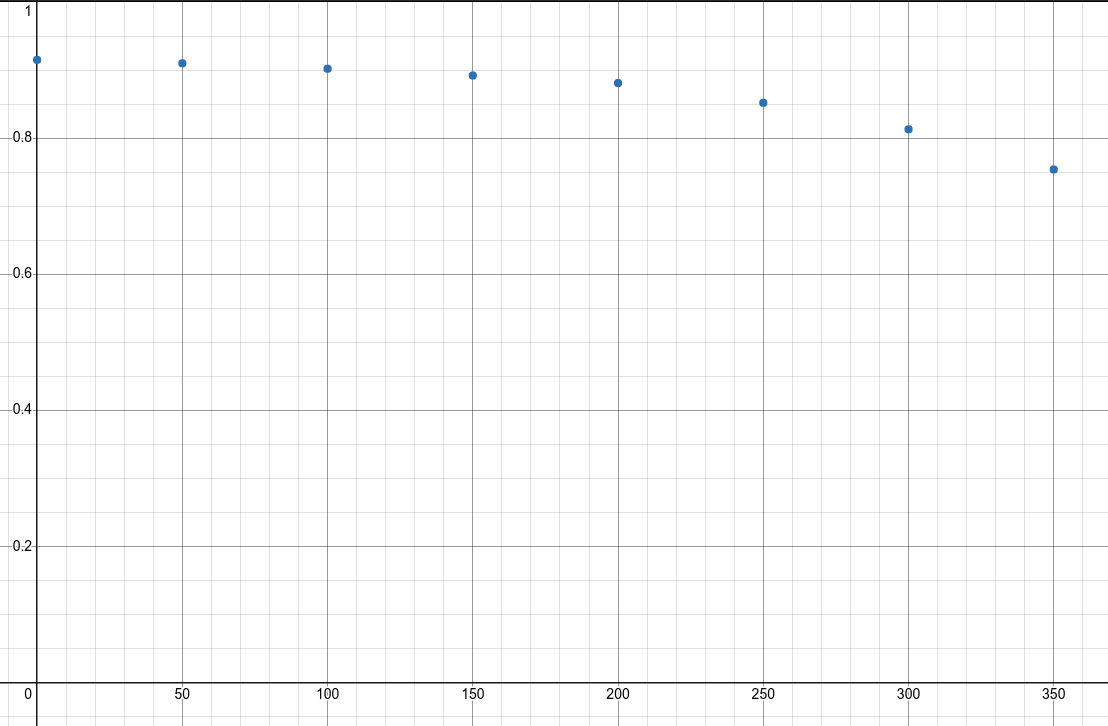
\includegraphics[width=.9\textwidth]{Figures/Lab\ Five/Case1}
  \caption{Plot for Part 5}
  \label{fig:10}
\end{figure}

\begin{figure}[H]
  \centering
  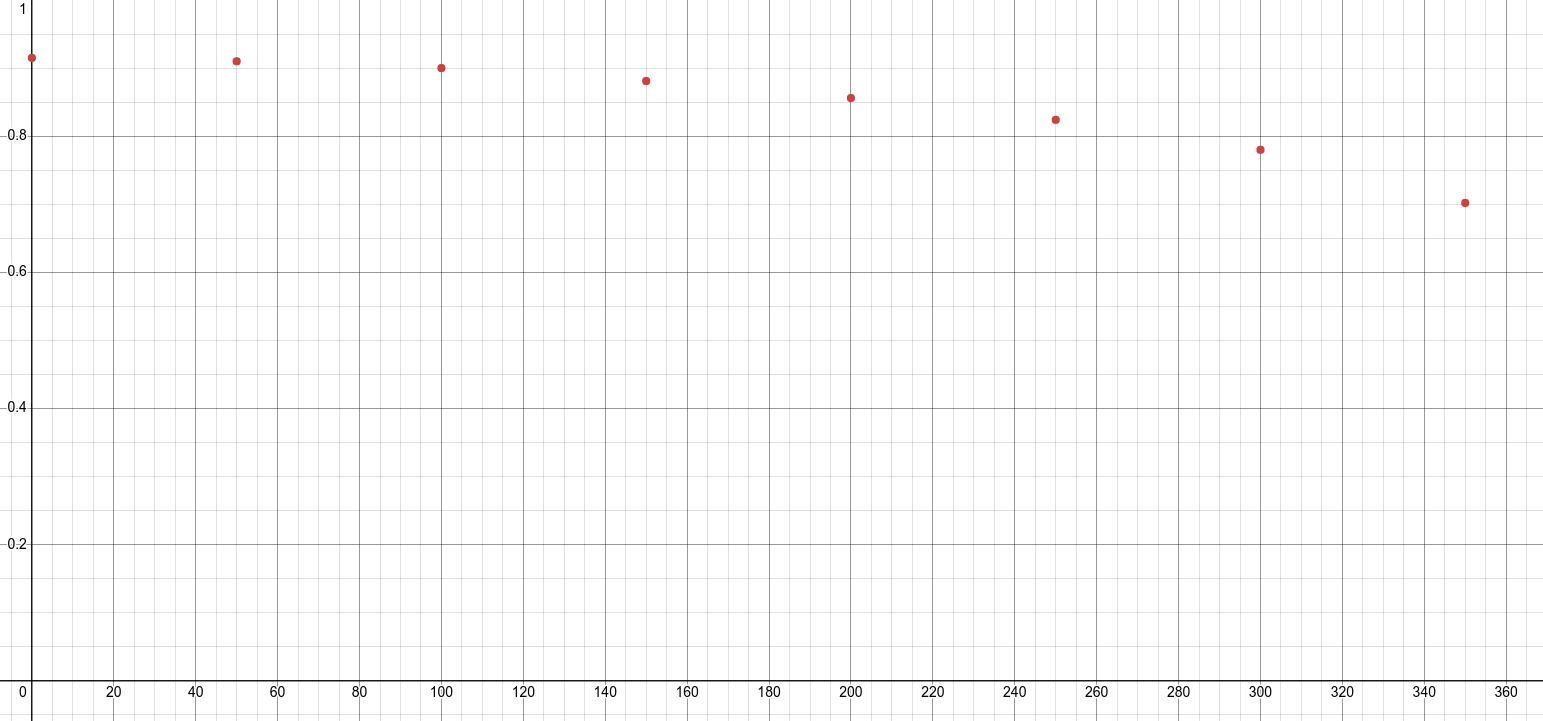
\includegraphics[width=.9\textwidth]{Figures/Lab\ Five/Case2}
  \caption{Plot for Part 6}
  \label{fig:11}
\end{figure}

Based on the PV plots, we may determine that the voltage is inversely related to the real power load, while reactive power load stays constant. This is the reason that reactive power injection is desirable, as it allows for voltage magnitude to remain more steady.

\subsection{How to Determine the Necessary Capacitance for Part 7}

Using the set up of the problem, we could simulate using the Newton-Raphsson method to determine the necessary capacitance value.

\subsection{Converting the Capacitance to Farads}

Given the base, we know that the capacitor base impedance is:

$$X_{b}=\frac{V^2}{Q}$$
$$X_{b}=\frac{(34.5\cdot10^3)^2}{100\cdot10^{6}\sin(60)j}$$
$$X_{b}=-13.744j[\si{\ohm}]$$

We know that capacitance may be written as:

$$X_C=\frac{1}{j\omega C}$$

This means:

$$\frac{1}{\omega C}=13.744$$
$$C=\frac{1}{13.744\omega}$$
$$C=\frac{1}{13.744(120\pi)}$$
$$C_b=193[\si{\micro\farad}]$$

Now that we know the base in farads, we may simply multiply by the per-unit value to get:

$$C=C_bC_{pu}$$
$$C=(1.51)(193\cdot10^{-6})$$
$$\boxed{C=291[\si{\micro\farad}]}$$

\end{document}
